% Aqui começa o capítulo de Introdução.
% Use o comando \label para definir um rótulo, 
% caso seja necessário referenciar esse capítulo
% posteriormente.
\chapter{Introdução}\label{chp:Introducao}

% Contextualização do problema baseada nos artigos de referência
A classificação precisa de uso e cobertura da terra (Land Use/Land Cover - LULC) representa um dos desafios mais importantes no monitoramento ambiental e na gestão sustentável de recursos naturais. O crescimento populacional e as mudanças climáticas intensificaram a necessidade de sistemas de monitoramento eficientes que possam detectar e quantificar mudanças na superfície terrestre em tempo hábil para subsidiar decisões de manejo e políticas ambientais \cite{Lou2024}.

Tradicionalmente, a classificação LULC baseava-se em imagens multiespectrais de satélites, que, embora úteis para análises em larga escala, apresentam limitações significativas em termos de resolução espacial e temporal para aplicações locais e regionais. A evolução da tecnologia de sensoriamento remoto trouxe as imagens hiperespectrais como uma alternativa promissora, oferecendo informações espectrais detalhadas com centenas de bandas espectrais contíguas que permitem uma caracterização mais precisa dos materiais e coberturas terrestres \cite{Shin2024}.

Recentemente, o advento dos Veículos Aéreos Não Tripulados (VANTs) ou drones equipados com sensores hiperespectrais revolucionou o campo do sensoriamento remoto hiperespectral. Esta combinação oferece vantagens únicas, incluindo alta flexibilidade operacional, capacidade de voo em baixas altitudes que minimiza interferências atmosféricas, custo-benefício superior em comparação com plataformas aerotransportadas tradicionais, e capacidade de aquisição de dados com alta resolução espacial e temporal \cite{Shin2024}.

\section{Motivação}\label{sec:motivacao}

A integração de sensores hiperespectrais em plataformas de drones apresenta oportunidades sem precedentes para aplicações em agricultura de precisão, monitoramento florestal, detecção de mudanças ambientais e gestão de recursos hídricos. Entretanto, esta integração também introduz desafios técnicos significativos que motivam esta pesquisa:

\subsection{Desafios do Processamento de Dados Hiperespectrais}
O processamento de imagens hiperespectrais de drones envolve múltiplas complexidades técnicas. Primeiro, o volume massivo de dados gerados pelos sensores hiperespectrais, com cada pixel contendo informações de centenas de bandas espectrais, resulta em datasets que podem exceder gigabytes por voo, demandando algoritmos eficientes de processamento e armazenamento.

Segundo, as distorções radiométricas e geométricas inerentes à aquisição por drones necessitam de correções precisas. Variações na irradiância solar, efeitos atmosféricos, ruído do sensor e instabilidades na orientação do drone podem comprometer significativamente a qualidade dos dados espectrais \cite{Shin2024}. O Método de Linha Empírica (Empirical Line Method - ELM) tem demonstrado eficácia na correção radiométrica, apresentando melhorias de 5-55\% na reflectância de painéis de referência \cite{Shin2024}.

\subsection{Limitações dos Métodos Tradicionais de Classificação}
Métodos tradicionais de classificação, como K-Nearest Neighbor (KNN) e Support Vector Machine (SVM), apresentam desempenho inadequado para o processamento de imagens hiperespectrais devido à alta dimensionalidade dos dados e à complexidade das relações espectrais. Estes métodos frequentemente ignoram informações espaciais importantes e requerem extração manual de características, resultando em classificações imprecisas e processos demorados \cite{Lou2024}.

\subsection{Potencial do Deep Learning}
Técnicas avançadas de deep learning, incluindo Redes Neurais Convolucionais (CNNs) e arquiteturas Transformer, têm demonstrado desempenho superior na classificação de imagens hiperespectrais, superando métodos tradicionais através da extração automática de características complexas e da exploração eficiente de informações espaciais e espectrais \cite{Lou2024}.

\section{Objetivos}\label{sec:objetivos}

\subsection{Objetivo Geral}
Desenvolver e validar uma metodologia integrada para classificação de uso e cobertura da terra utilizando imagens hiperespectrais coletadas por drones, aplicando técnicas avançadas de processamento de dados e algoritmos de deep learning para aplicações em agricultura de precisão.

\subsection{Objetivos Específicos}
\begin{enumerate}
    \item Implementar um pipeline completo de pré-processamento de imagens hiperespectrais de drones, incluindo correções radiométricas através do Método de Linha Empírica (ELM) e correções geométricas utilizando pontos de controle terrestres
    
    \item Desenvolver e avaliar algoritmos de redução de dimensionalidade (PCA, t-SNE) otimizados para dados hiperespectrais de alta dimensionalidade coletados por drones
    
    \item Implementar e comparar arquiteturas de deep learning (CNNs 2D/3D e Transformers) para classificação automática de diferentes classes de uso e cobertura da terra
    
    \item Validar a metodologia proposta através de experimentos com dados reais coletados em diferentes condições ambientais e tipos de cobertura vegetal
    
    \item Quantificar melhorias na acurácia de classificação em comparação com métodos tradicionais, estabelecendo métricas de desempenho objetivas
    
    \item Desenvolver diretrizes práticas para implementação da metodologia em aplicações reais de agricultura de precisão e monitoramento ambiental
\end{enumerate}

\section{Contribuições Esperadas}\label{sec:contribuicoes}

Esta pesquisa contribui para o avanço do estado da arte em várias dimensões:

\subsection{Contribuições Metodológicas}
\begin{itemize}
    \item \textbf{Pipeline Integrado de Processamento}: Primeira implementação sistemática de um pipeline completo que integra correções radiométricas e geométricas específicas para dados hiperespectrais de drones com técnicas avançadas de deep learning
    
    \item \textbf{Otimização de Algoritmos}: Desenvolvimento de algoritmos otimizados de redução de dimensionalidade e classificação específicos para as características únicas dos dados hiperespectrais coletados por drones
    
    \item \textbf{Metodologia de Validação}: Estabelecimento de protocolos padronizados para validação de sistemas de classificação LULC baseados em drones hiperespectrais
\end{itemize}

\subsection{Contribuições Técnicas}
\begin{itemize}
    \item \textbf{Implementações Otimizadas}: Código-fonte aberto e reproduzível de algoritmos de processamento hiperespectral otimizados para aplicações em tempo real
    
    \item \textbf{Base de Dados Referencial}: Criação de dataset anotado de imagens hiperespectrais de drones para diferentes tipos de cobertura vegetal em condições brasileiras
    
    \item \textbf{Ferramentas de Análise}: Desenvolvimento de ferramentas computacionais para análise automática de acurácia e interpretação de resultados de classificação
\end{itemize}

\subsection{Contribuições Aplicadas}
\begin{itemize}
    \item \textbf{Agricultura de Precisão}: Diretrizes práticas para implementação de sistemas de monitoramento baseados em drones hiperespectrais para detecção precoce de estresses em culturas
    
    \item \textbf{Monitoramento Ambiental}: Metodologia validada para detecção de mudanças na cobertura vegetal e identificação de áreas degradadas
    
    \item \textbf{Transferência de Tecnologia}: Protocolos operacionais para implementação da tecnologia em instituições de pesquisa e empresas do setor agrícola
\end{itemize}

\section{Organização do Texto}\label{sec:organizacao}

Esta dissertação está estruturada em sete capítulos que cobrem desde a fundamentação teórica até a validação experimental da metodologia proposta:

\begin{itemize}
    \item \textbf{\Capitulo{chp:levantamento}}: Apresenta uma revisão abrangente da literatura sobre classificação LULC com imagens hiperespectrais, tecnologias de drones para sensoriamento remoto, técnicas de correção radiométrica e geométrica, e aplicações de deep learning em processamento de imagens hiperespectrais.
    
    \item \textbf{\Capitulo{chp:metodologia}}: Detalha a metodologia experimental proposta, incluindo a descrição do pipeline de processamento, algoritmos implementados, configuração dos experimentos e métricas de avaliação utilizadas.
    
    \item \textbf{\Capitulo{chp:dados}}: Descreve os datasets utilizados, procedimentos de coleta de dados em campo, especificações dos equipamentos e protocolos de aquisição de imagens hiperespectrais com drones.
    
    \item \textbf{\Capitulo{chp:processamento}}: Apresenta os algoritmos de pré-processamento implementados, incluindo correções radiométricas e geométricas, técnicas de redução de dimensionalidade e preparação dos dados para classificação.
    
    \item \textbf{\Capitulo{chp:resultados}}: Apresenta os resultados experimentais obtidos, incluindo análises quantitativas de acurácia, comparações entre diferentes algoritmos e validação da metodologia proposta.
    
    \item \textbf{\Capitulo{chp:discussao}}: Analisa e discute os resultados obtidos, identifica limitações da metodologia, compara com trabalhos relacionados e discute implicações práticas dos achados.
    
    \item \textbf{\Capitulo{chp:conclusoes}}: Sumariza as principais conclusões, contribuições da pesquisa, limitações identificadas e direções para trabalhos futuros.
\end{itemize}

\section{Estrutura dos Experimentos}\label{sec:estrutura_experimentos}

Os experimentos foram estruturados em três fases principais para validação sistemática da metodologia proposta:

\subsection{Fase 1: Validação de Pré-processamento}
Avaliação da eficácia das correções radiométricas e geométricas através de análise comparativa de dados antes e após processamento, utilizando métricas de correlação espectral e precisão geométrica.

\subsection{Fase 2: Comparação de Algoritmos de Classificação}
Comparação sistemática entre métodos tradicionais (SVM, Random Forest) e técnicas de deep learning (CNN 2D/3D, Transformers) utilizando métricas padronizadas de acurácia, precisão, recall e F1-score.

\subsection{Fase 3: Validação em Condições Reais}
Teste da metodologia completa em diferentes cenários de aplicação, incluindo variações sazonais, tipos de culturas e condições ambientais, para verificação da robustez e generalização dos resultados.

Os capítulos subsequentes detalham cada um destes aspectos, fornecendo uma base sólida para compreensão e reprodução da metodologia desenvolvida.

A seguir, estão alguns exemplos para os elementos mais comuns em textos acadêmicos, \ie tabelas, equações e figuras. 

\section{Exemplos de Tabelas e Equações}\label{sec:exemplostabelas}
Aqui um exemplo de como referenciar a \Tabela{tab:tabela_1}. Note que é preciso definir um rótulo (\textit{label}) dentro do comando de definição da tabela.

% Veja a seguir um exemplo de Tabela.
% Você pode usar o site http://www.tablesgenerator.com
% para gerar as tabelas em LaTeX.
\begin{table}[!htp]
\caption[Legenda curta da tabela]{Legenda longa e mais detalhada da tabela.}
\label{tab:tabela_1}
\begin{center}
\begin{tabular}{cc}
\toprule % Linha superior
Coluna 1 & Coluna2 \\ \midrule % Linha do meio 
a & b \\
c & d \\
e & f \\\bottomrule % Linha inferior
\end{tabular}
\end{center}
\end{table}

As tabelas mais complexas podem ser feitas com ajuda no site \href{http://www.tablesgenerator.com}{http://www.tables\-ge\-ne\-ra\-tor.com}.

Veja um exemplo de equação no próprio texto, \eg, $x=\frac{\sqrt{a^{2}+b^{2}}}{\sigma}$.  Se você preferir, pode escrever a equação de forma estendida, conforme a \Equacao{eq:teste} a seguir. Note que o rótulo é colocado automaticamente.

\begin{equation}
x=\frac{\sqrt{a^{2}+b^{2}}}{\sigma}
\label{eq:teste}
\end{equation}


Você também pode obter ajudar para escrever as equações em \LaTeX no site \url{http://www.codecogs.com/latex/eqneditor.php}.

% Note que podemos incluir automaticamente alguns termos na lista de abreviaturas e siglas no pré-texto. Veja exemplos a seguir no código fonte. 

% A sigla \Sigla{abêcê}{ABC} aparecerá automaticamente na lista de abreviaturas e siglas no pré-texto. Do mesmo modo, podemos usar o comando \SiglaHifen{xisipsilonzê}{XYZ} separado por hífen ao invés de aparecer entre parênteses.

Veja na \Secao{sec:exemplo_secao} a seguir como referenciar uma seção. Também será preciso definir um rótulo (\textit{label}) logo após o comando \texttt{\textbackslash section}.

% Aqui começa uma Seção.
% Use o comando \label para definir um rótulo, 
% caso seja necessário referenciar essa seção
% posteriormente.
\section{Exemplo de seção}\label{sec:exemplo_secao} 
Agora observe como se faz uma citação de artigo científico em periódico \cite{Gradvohl2014c}. De acordo com \textcite{Gradvohl2016}, essa é uma citação direta. Se for citar mais de um trabalho, faça da seguinte forma \cite{Caldana2017,Gradvohl2015}. As referências bibliográficas estão no arquivo \texttt{bibliografia.bib}. Outros exemplos de citações também se encontram nesse arquivo.

Veja a seguir o comando para criar uma figura e o resultado, na \Figura{fig:xwing}. Note, no código fonte, que no comando \texttt{caption} podemos estabelecer uma \enquote{legenda curta} para aparecer na Lista de Figuras. A legenda curta é opcional.

\begin{figure}[!htb]
\centering
% As figuras estão na pasta figuras.
% Se seu texto estiver demorando muito para compilar, use figuras no formato PDF ou PNG.
% Observe, no comando includegraphics que você pode estabelecer uma proporção para a figura.
% Nesse caso, a figura tem uma proporção equivalente à metade (0.5) da largura do texto (\textwidth)
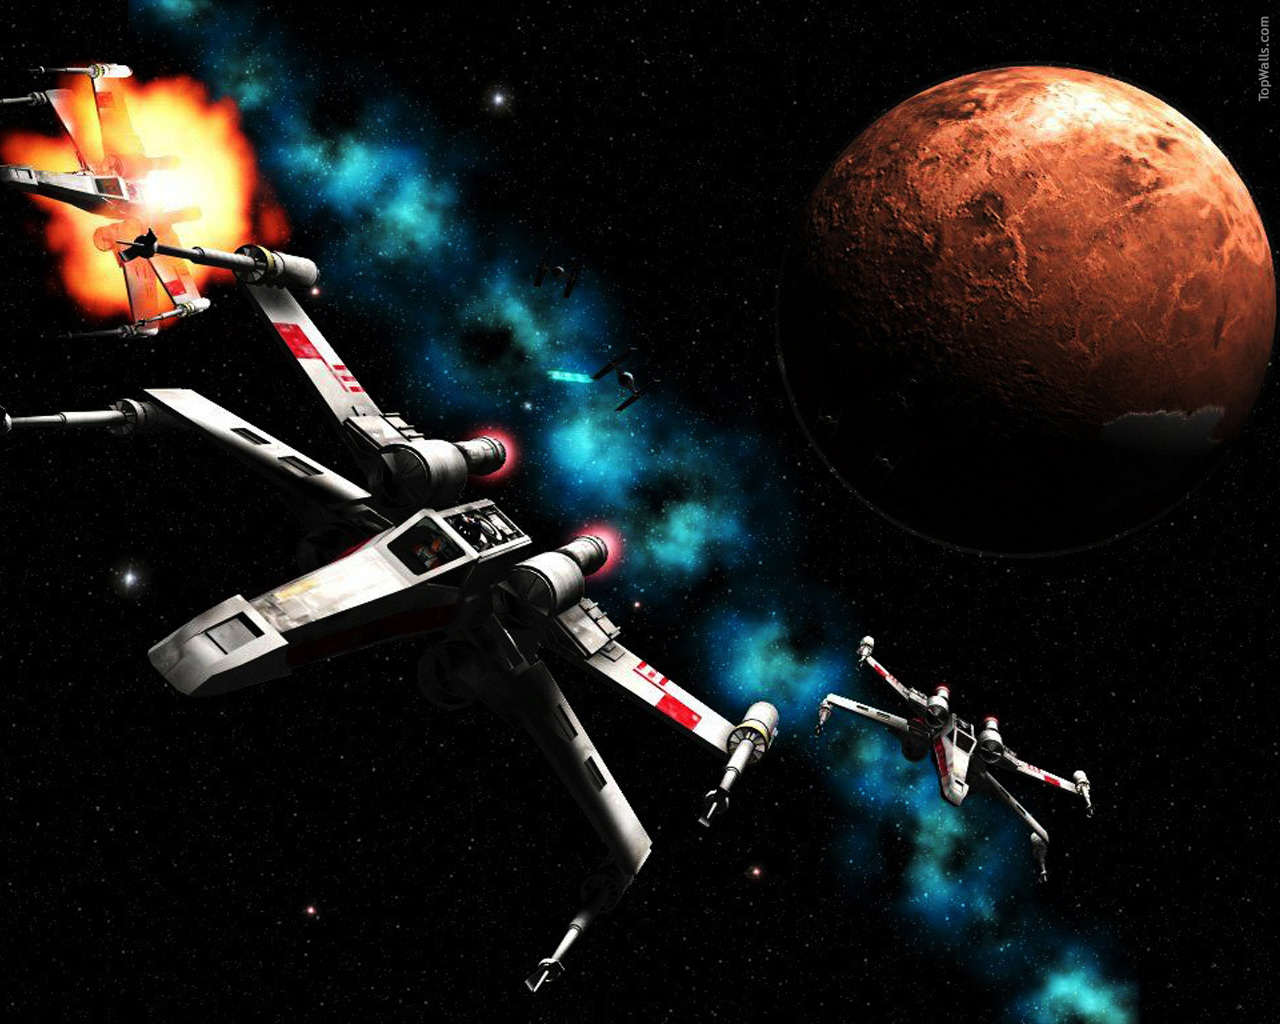
\includegraphics[width=0.5\textwidth]{starwars21280.jpg}
\caption[Legenda curta de figura]{Legenda mais extensa de figura.}
\label{fig:xwing}
\end{figure}

Dica importante: sempre que possível, use figuras no formato PDF. De acordo com o Overleaf, isso acelera a compilação do texto, sem perder a qualidade da figura. 

\subsection{Exemplo de subseção}\label{subsec:exemploSubsec}
É importante evitar chegar a esse nível de subseção. Dois níveis são suficientes. Use essa opção em último caso, apenas.


\subsection{Exemplo de adição de siglas}\label{subsec:siglas}
Para adicionar uma sigla ou abreviatura na lista de siglas e abreviaturas, use o comando ``\texttt{\textbackslash{}Sigla\{nome por extenso\}\{abreviatura\}}'' ou ``\texttt{\textbackslash{}SiglaHifen\{nome por} \texttt{ex\-ten\-so\}\{abreviatura\}}'' para adicionar a sigla com hífen. 
Por exemplo, respectivamente, \Sigla{Ácido Desoxirribonucleico}{DNA} ou \SiglaHifen{Ácido Ribonucleico}{RNA}. A lista de siglas é adicionada automaticamente.

\section{Comandos opcionais para facilitar}\label{sec:comandosOpc}
Este modelo também criou alguns comandos adicionais não apenas para facilitar o trabalho de quem escreve, mas também para manter uma formatação mais consistente.

Entre esses comandos estão o \texttt{\textbackslash{}ie} que inclui a abreviatura ``\ie'' no texto (equivalente ao ``isto é''). Usar esse comando vai garantir que a abreviatura não se separe entre linhas e que o espaço entre o `.' e a próxima letra seja fixo. O mesmo vale para os comandos \texttt{\textbackslash{}eg} que inclui a abreviatura ``\eg'' e \texttt{\textbackslash{}pex} que inclui a abreviatura ``\pex''.

Também existem os comandos \texttt{\textbackslash{}Capitulo\{rótulo do capítulo\}}, \texttt{\textbackslash{}Equacao\{ró\-tu\-lo da equação\}}, \texttt{\textbackslash{}Figura\{rótulo da figura\}}, \texttt{\textbackslash{}Secao\{rótulo da seção\}} e \texttt{\textbackslash{}Tabela\{rótulo da tabela\}}. Esses comandos inserem referências para os respectivos elementos. Além disso, no próprio texto aparece a \textit{string} (``Capítulo'', ``Equação'', ``Figura'' etc) seguida da referência já com o link. Por exemplo, \Secao{sec:exemplo_secao}. Sugere-se a utilização desses comandos para referenciar os respectivos elementos ao invés do comando \texttt{\textbackslash{}ref\{rótulo\}}. Assim, o texto ficará mais uniforme. 

É possível também usar esses comandos nas versões no plural para conjuntos de referências. Por exemplo, para referenciar várias seções, você pode utilizar o comando \texttt{\textbackslash{}secoes\{ró\-tu\-lo\_1, rótulo\_2, rótulo\_3\}}.

Por exemplo, suponha que queiramos referenciar as \secoes{sec:exemplostabelas,sec:exemplo_secao,subsec:siglas}.